\documentclass[12pt]{beamer}
\usepackage[T2A]{fontenc} 
\usepackage[utf8]{inputenc} 
\usepackage{algorithm}
\usepackage{algorithmic}
\usepackage[english, ukrainian]{babel} 
\mode<presentation>{
	\usetheme{CambridgeUS}
    \setbeamercovered{transparent}
}
%% preamble
\title{Ієрархічні матриці}
\author{Солук Олена}
\date[ 2017]
{\large{Львівський національний університет імені І.Франка}}
\begin{document}
\begin{frame}
	\titlepage
\end{frame}
%% normal frame
\begin{frame}{Зміст}
\begin{block}{}
	1. Сluster tree i block cluster tree.\\
	2. Умова допустимості.\\
	3. Означення $\mathcal{H}$-матриці.\\
	4. Модельна задача BEM.\\
	5. Програмна репрезентація $\mathcal{H}$-матриці.
\end{block}	
\end{frame}

\begin{frame}
\frametitle{Cluster Tree}
	\begin{block}{Означення}
		Дерево $\mathbb{T}_{I}$ називається cluster tree над множиною індексів $I$ з $root(\mathbb{T}_{I})=I$, якщо наступні умови виконуються:
			\begin{enumerate}
				\item[-] $I \in V$ є коренем $\mathbb{T}_{I}$ i $\forall v \in V,v\not=\O \Rightarrow v\subseteq I$.
				\item[-] Якщо $v\in V$ не є листком ($S(v)\not=\O$), то він рівний об'єднанню своїх синів, тобто $v=\bigcup_{w\in S(v)}w$.
			\end{enumerate}
	\end{block}
	\begin{block}{}
		$v\in V$ називають кластером.
	\end{block}
	\begin{block}{}
		В одновимірному випадку cluster tree - збалансоване бінарне дерево.
	\end{block}
\end{frame}
\begin{frame}{Приклад побудови cluster tree}
	\begin{block}{}
		$$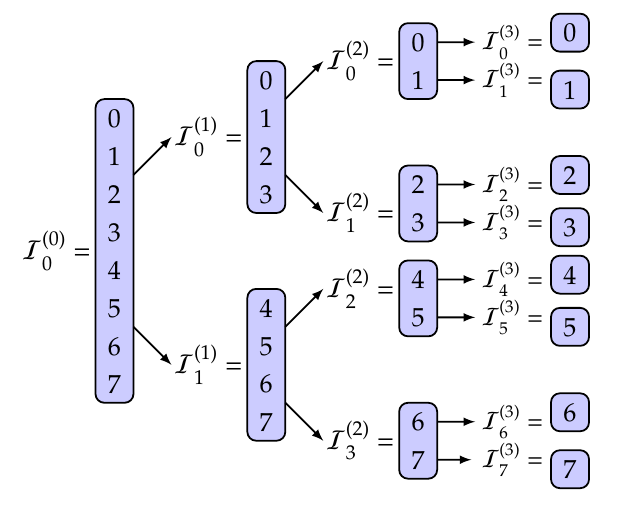
\includegraphics[scale=0.48]{1_0}$$
	\end{block}
\end{frame}
\begin{frame}
\frametitle{Block Cluster Tree}
	\begin{block}{Означення}
	Нехай $\mathbb{T}_{I}$ і $\mathbb{T}_{J}$ - cluster trees над множинами індексів $I$ та $J$ відповідно. Cluster tree $\mathbb{T}_{I\times J}=\mathbb{T}_{\mathbb{T}_{I}\times \mathbb{T}_{J}}=(V,E)$ називається block cluster tree над добутком множини індексів $I\times J$, якщо $\forall v\in V$ виконуються наступні умови:
		\begin{enumerate}
			\item[-] $\mathbb{T}^{(0)}_{I\times J}=I\times J$
			\item[-] Якщо $v\in \mathbb{T}^{(l)}_{I\times J}$, то існують $\tau \in \mathbb{T}^{(l)}_I$ i $\sigma \in \mathbb{T}^{(l)}_J$ такі, що $v=\tau \times \sigma$.
			\item[-] Для синів $v=\tau \times \sigma$, де  $\tau \in \mathbb{T}_I$ i $\sigma \in \mathbb{T}_J$ виконується
			\newline
			S(v)=$\begin{cases}
			$\O,$\text{якщо $S(\tau)=\O$ або $S(\sigma)=\O$}\\
			$$\{\tau^{\prime}\times\sigma^{\prime} : \tau^{\prime} \in S(\tau),\sigma^{\prime} \in S(\sigma)\}$,$\text{інакше}
			\end{cases}$
		\end{enumerate}
	\end{block}
\end{frame}

\begin{frame}
\frametitle{Умова допустимості}
	\begin{block}{Означення}
	Умова допустимості є булівською функцією 
		$$Adm:\mathbb{T}_{I\times J}\rightarrow\{true,false\}$$
		для якої виконуються умови
		$$Adm(b)\Rightarrow Adm(b'),\quad\text{для всіх синів } b'\subseteq b\in \mathbb{T}_{I\times J} $$
		
		$$Adm(b)=true, \quad\text{для всіх листків } b\in \mathbb{T}_{I\times J}$$
	\end{block}
	
\end{frame}

\begin{frame}
	\begin{block}{}
	 В подальшому для одновимірної проблеми ми будемо використовувати стандартну умову допустимості в такому вигляді
		\newline
		$$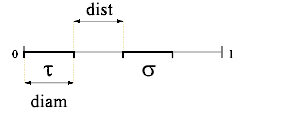
\includegraphics{1_2}$$
		$$diam(\tau)\le dist(\tau,\sigma)$$
	\end{block}
\end{frame}

\begin{frame}{Приклад побудови block cluster tree}
	\begin{block}{}
		\centering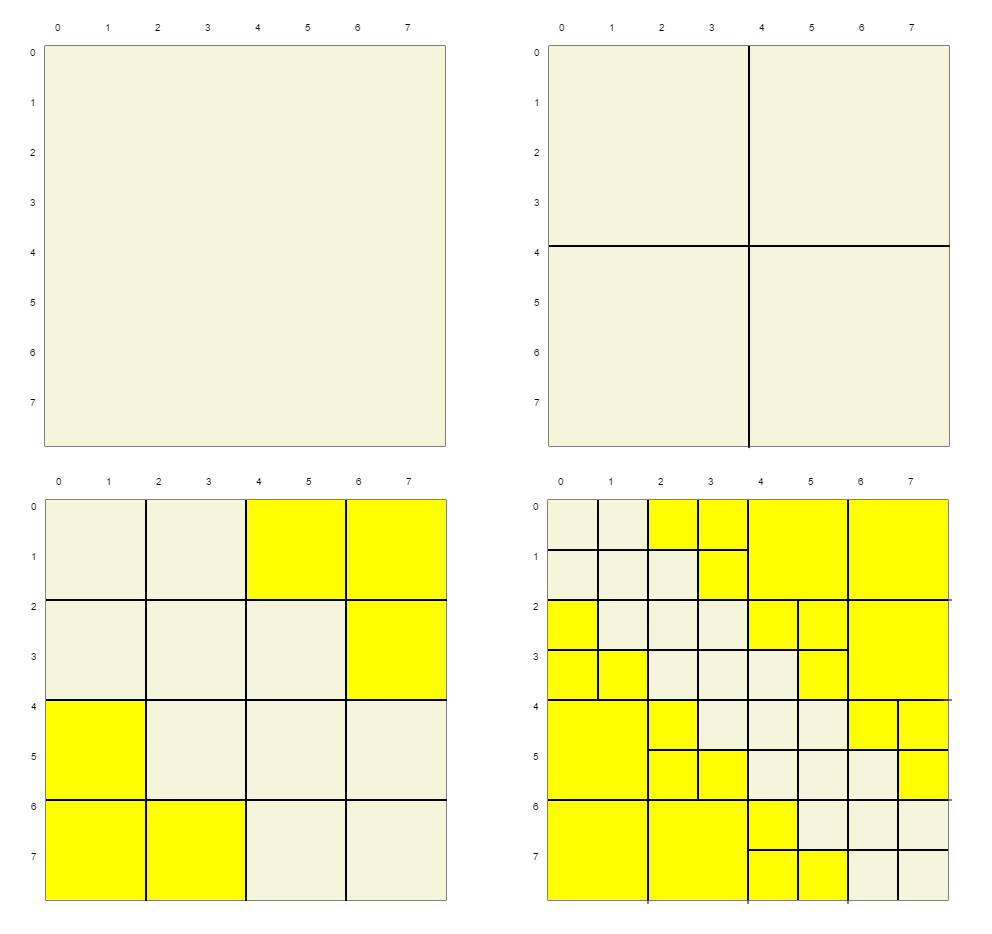
\includegraphics[scale=0.27]{1_3}
	\end{block}
\end{frame}
\begin{frame}
\frametitle{Означення $\mathcal{H}$-матриці}
	\begin{block}{Означення}
		Нехай $\mathbb{T}_{I\times I}$ - block cluster tree над множиною індексів $I$. Означаємо множину $\mathcal{H}$-матриць як
			$$\mathcal{H}(\mathbb{T}_{I\times I},k):=\{M\in\mathbb{R}^{I\times I}|rank(M|_{t\times s})\le k \text{ для всіх}$$ $$\text{допустимих листків } t\times s \text{ дерева } \mathbb{T}_{I\times I} \}$$
	\end{block}
\end{frame}
\begin{frame}{BEM}
	\begin{block}{}
		Нехай задано функцію $F:[0,1]\rightarrow \mathbb{R}$. Шукаємо функцію $u:[0,1]\rightarrow \mathbb{R}$, яка задовільняє наступне інтегральне рівняння: $$\int_{0}^{1}\ln|x-y|u(y)dy=F(x), x\in[0,1] \eqno(1)$$
			де $g(x,y)=\ln|x-y|$ називається ядром інтегрального рівняння
	\end{block}
	\begin{block}{Метод Гальоркіна}
	$V_n=span\{\varphi_0,\dots,\varphi_{n-1}\}$
		
		$$\int_{0}^{1}\int_{0}^{1}\varphi_i(x)\ln|x-y|u(y)dydx=\int_{0}^{1}\varphi_i(x)F(x)dx\eqno(2) $$
		
		
	\end{block}
\end{frame}
\begin{frame}{}
	\par Потрібно знайти $u_n$ в просторі $V_n$:
			$$u_n=\sum_{j=0}^{n-1}u_j\varphi_j\eqno(3)$$
			таке, що вектор коефіцієнтів $u$ є розв'язком лінійної системи $$Gu=f$$
			$$G_{ij}=\int_{0}^{1}\int_{0}^{1}\varphi_i(x)\ln|x-y|\varphi_j(y)dydx\eqno(4)$$ 
			$$f_i=\int_{0}^{1}\varphi_i(x)F(x)dx$$
\end{frame}
\begin{frame}
	\begin{block}{}
	Базисні функції визначені як
		\newline 
		\begin{equation*}
		\varphi_i(x)=\begin{cases}
					1,\quad\text{якщо $\frac{i}{n}\le x\le \frac{i+1}{n}$}\\
					0,\quad\text{інакше}
					\end{cases}
		\end{equation*}
	\end{block}
	\begin{block}{}
	Шукаємо наближену матрицю $\tilde{G}$. Для цього заміняємо ядро $g(x,y)=\ln|x-y|$ на розкладене ядро $$\tilde{g}(x,y)=\sum_{v=0}^{k-1}g_v(x)h_v(y)\eqno(5)$$
	Будуємо локальні наближення на підобластях $[0,1]\times[0,1]$, де $g$ є гладкою: $\tau:=[a,b]$, $\sigma:=[c,d]$, $\tau\times\sigma\subset[0,1]\times[0,1]$, $\tau\cap\sigma=\O$.
	 $x_0:=(a+b)/2$
	\end{block}
\end{frame}

\begin{frame}
\frametitle{Наближення низького рангу блоків матриці}
	\begin{block}{}
		$$\tilde{G}_{ij}=\int_{0}^{1}\int_{0}^{1}\varphi_i(x)\tilde{g}(x,y)\varphi_j(y)dydx = $$
		$$\int_{0}^{1}\int_{0}^{1}\varphi_i(x)\sum_{v=0}^{k-1}g_v(x)h_v(y)\varphi_j(y)dydx $$
		$$=\sum_{v=0}^{k-1}(\int_{0}^{1}\varphi_i(x)g_v(x)dx)(\int_{0}^{1}\varphi_j(y)h_v(y)dy)$$
	\end{block}
	\begin{block}{Факторизований вигляд підматриці}
		$$G|_{t\times s}=AB^\top,\quad A\in\mathbb{R}^{t\times\{0,\dots,k-1\}},\quad B\in\mathbb{R}^{s\times\{0,\dots,k-1\}}$$
			$$A_{iv}:=\int_{0}^{1}\varphi_i(x)g_v(x)dx, \quad B_{jv}:=\int_{0}^{1}\varphi_j(y)h_v(y)dy\eqno(5)$$
	\end{block}
\end{frame}
\begin{frame}
\frametitle{Програмна репрезентація $\mathcal{H}$-матриці.}
	\begin{block}{Недопустимі листки}
	$$\tilde{G_{ij}}:=\int_{0}^{1}\int_{0}^{1}\varphi_i(x)\ln|x-y|\varphi_j(y)dydx$$$$=\int_{i/n}^{(i+1)/n}\int_{j/n}^{(j+1)/n}ln|x-y|dydx$$
	\end{block}
	\begin{block}{Репрезентація fullmatrix}
	Кажуть, що матриця $M$ розмірності $n\times m$ зберігається у вигляді fullmatrix, якщо її елементи $M_{ij}$ зберігаються як дійсні числа у масиві довжиною $mn$ в стовпцевому порядку
			$$M_{11},\dots,M_{n1},M_{12},\dots,M_{n2},\dots,M_{1m},\dots,M_{nm}$$
	\end{block}
\end{frame}
\begin{frame}
	\begin{block}{Допустимі листки}
	$$\tilde{G}|_{t\times s}:=AB^\top$$
		$$A_{iv}:=\int_{i/n}^{(i+1)/n}(x-x_0)^vdx$$
		\begin{equation*}
			B_{jv}:=\begin{cases}
						(-1)^{v+1}v^{-1}\int_{j/n}^{(j+1)/n}(x_0-y)^{-v}dy,\quad\text{якщо $v>0$}\\
						\int_{j/n}^{(j+1)/n}\ln|x_0-y|dy,\quad\text{якщо $v=0$}
					\end{cases}
		\end{equation*}
	\end{block}
	\begin{block}{Репрезентація rkmatrix}
		Кажуть, що матриця $M$ розмірності $n\times m$ найбільшого рангу $k$ зберігається у вигляді rkmatrix, якщо вона зберігається у факторизованій формі $M=AB^\top$, де обидві матриці $A\in\mathbb{R}^{n\times k}$ i $B\in \mathbb{R}^{m\times k}$ зберігаються як масиви (в стовпцевому порядку).
	\end{block}
\end{frame}
\begin{frame}
	\begin{block}{Репрезентація $\mathcal{H}$-матриці}
	 Нехай $\mathbb{T}_{I\times I}$ - block cluster tree над множиною індексів $I$. Кажуть, що матриця $M\in\mathcal{H}(\mathbb{T}_{I\times I},k)$ зберігається в $\mathcal{H}$-matrix репрезентації, якщо підматриці, що відповідають недопустимим листкам, зберігаються у вигляді fullmatrix, а ті, що відповідають допустимим листкам - у вигляді rkmatrix. 
	\end{block}
	\begin{block}{}
		
		$$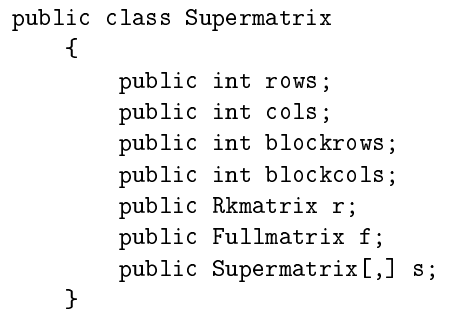
\includegraphics[scale=0.48]{1_5}$$
		
	\end{block}
\end{frame}
\begin{frame}
	\begin{center}
		\Huge{Дякую за увагу!}
	\end{center}
\end{frame}

\end{document}
